% !TEX encoding = UTF-8 Unicode
%*********************************************
\chapter{Overview}\label{ch:introduction}

%*********************************************
\openepigraph{As far as the laws of mathematics refer to reality, they are not certain, and as far as they are certain, they do not refer to reality.}{Albert Einstein}

\section{Context}

\subsection{A Tale of Babylonians and Greeks}



\sidefigure{feynman}{0}{Richard Feynman, Nobel laureate physicist.\protect\footnotemark}

\protect\footnotetext{Except when otherwise stated, all images were created by the author.}
Richard Feynman (\cref{fig:feynman}) used to lecture this story~\cite{feynman:1994}: Babylonians were pioneers in mathematics; Yet, the Greeks took the credit. We are used to the Greek way of doing Math: start from the most basic axioms and build up a knowledge system. Babylonians were quite the opposite; they were pragmatic. No knowledge was considered more fundamental than others, and there was no urge to derive proofs in a particular order. Babylonians were concerned with the phenomena, Greeks with the ordinance. In Feynman's view, science is constructed in the Babylonian way. There is no fundamental truth. Theories try to connect dots from different pieces of knowledge. Only as science advances one can worry about reformulation, simplification and ordering. Scientists are Babylonians; mathematicians are Greeks.

Mathematics and science are both tools for knowledge acquisition. Also, they are social constructs, as both rely on peer-reviewing. They are pretty different, however.

Science is empiric, based on facts collected from \textbf{experience}. When physicists around the world measured events that corroborated Newton's \emph{``Law of Universal Gravitation''}, they did not prove it correct; they just made his theory more and more plausible. Still, it was needed only one experiment to show that Einstein's \emph{Relativity Theory} was even more believable. In contrast, we can and do prove things in mathematics.

In mathematics, knowledge is absolute truth, and the way one builds new knowledge with it, its inference method, is deduction.  Mathematics is language, a formal one, a tool to precisely communicate some kinds of thoughts. As it happens with natural languages, there is beauty in it. The mathematician expands the boundaries of expression in this language, and Greeks were poets. Even though Babylonians were first in finding mathematical truths, the Greeks invented Mathematics as epistemology.

In science, there are no axioms: a falsifiable hypothesis/theory is proposed, and logical conclusions (predictions) from the theory are empirically tested. Despite inferring hypotheses by induction, there is no influence of psychology in the process. A tested hypothesis is not absolute truth. A hypothesis is never verified, only falsified by experiments~\cite[p. 31-50]{popper:2004}. Scientific knowledge is belief justified by experience; there are degrees of plausibility.

Understanding the epistemic contrast between mathematics and science will help us understand the past of \acf{AI} and avoid some perils in its future. This contrast will be a recurrent theme in this dissertation.

\subsection{The importance of theoretical development} In science, we collect facts, but they need interpretation. Science is a narrative of how we understand the world\cite{gleiser:2018}. The logical conclusion from the hypothesis that predicts some behaviour in nature gives a plausible meaning to what we observed.

To illustrate, take the ancient human desire of flying. Since antiquity, there have been stories of men strapping wings to themselves and attempting to fly by jumping from a tower and flapping those wings like birds (see \cref{fig:goya}). While concepts like lift, stability, and control were poorly understood, most human flight attempts ended in severe injury or even death. It did not matter how much evidence, how many hours of seeing different animals flying, those ludicrous brave men experienced; the meaning they took from what they saw was wrong, and their predictions incorrect.
\begin{figure}
	[ht!] \centering
	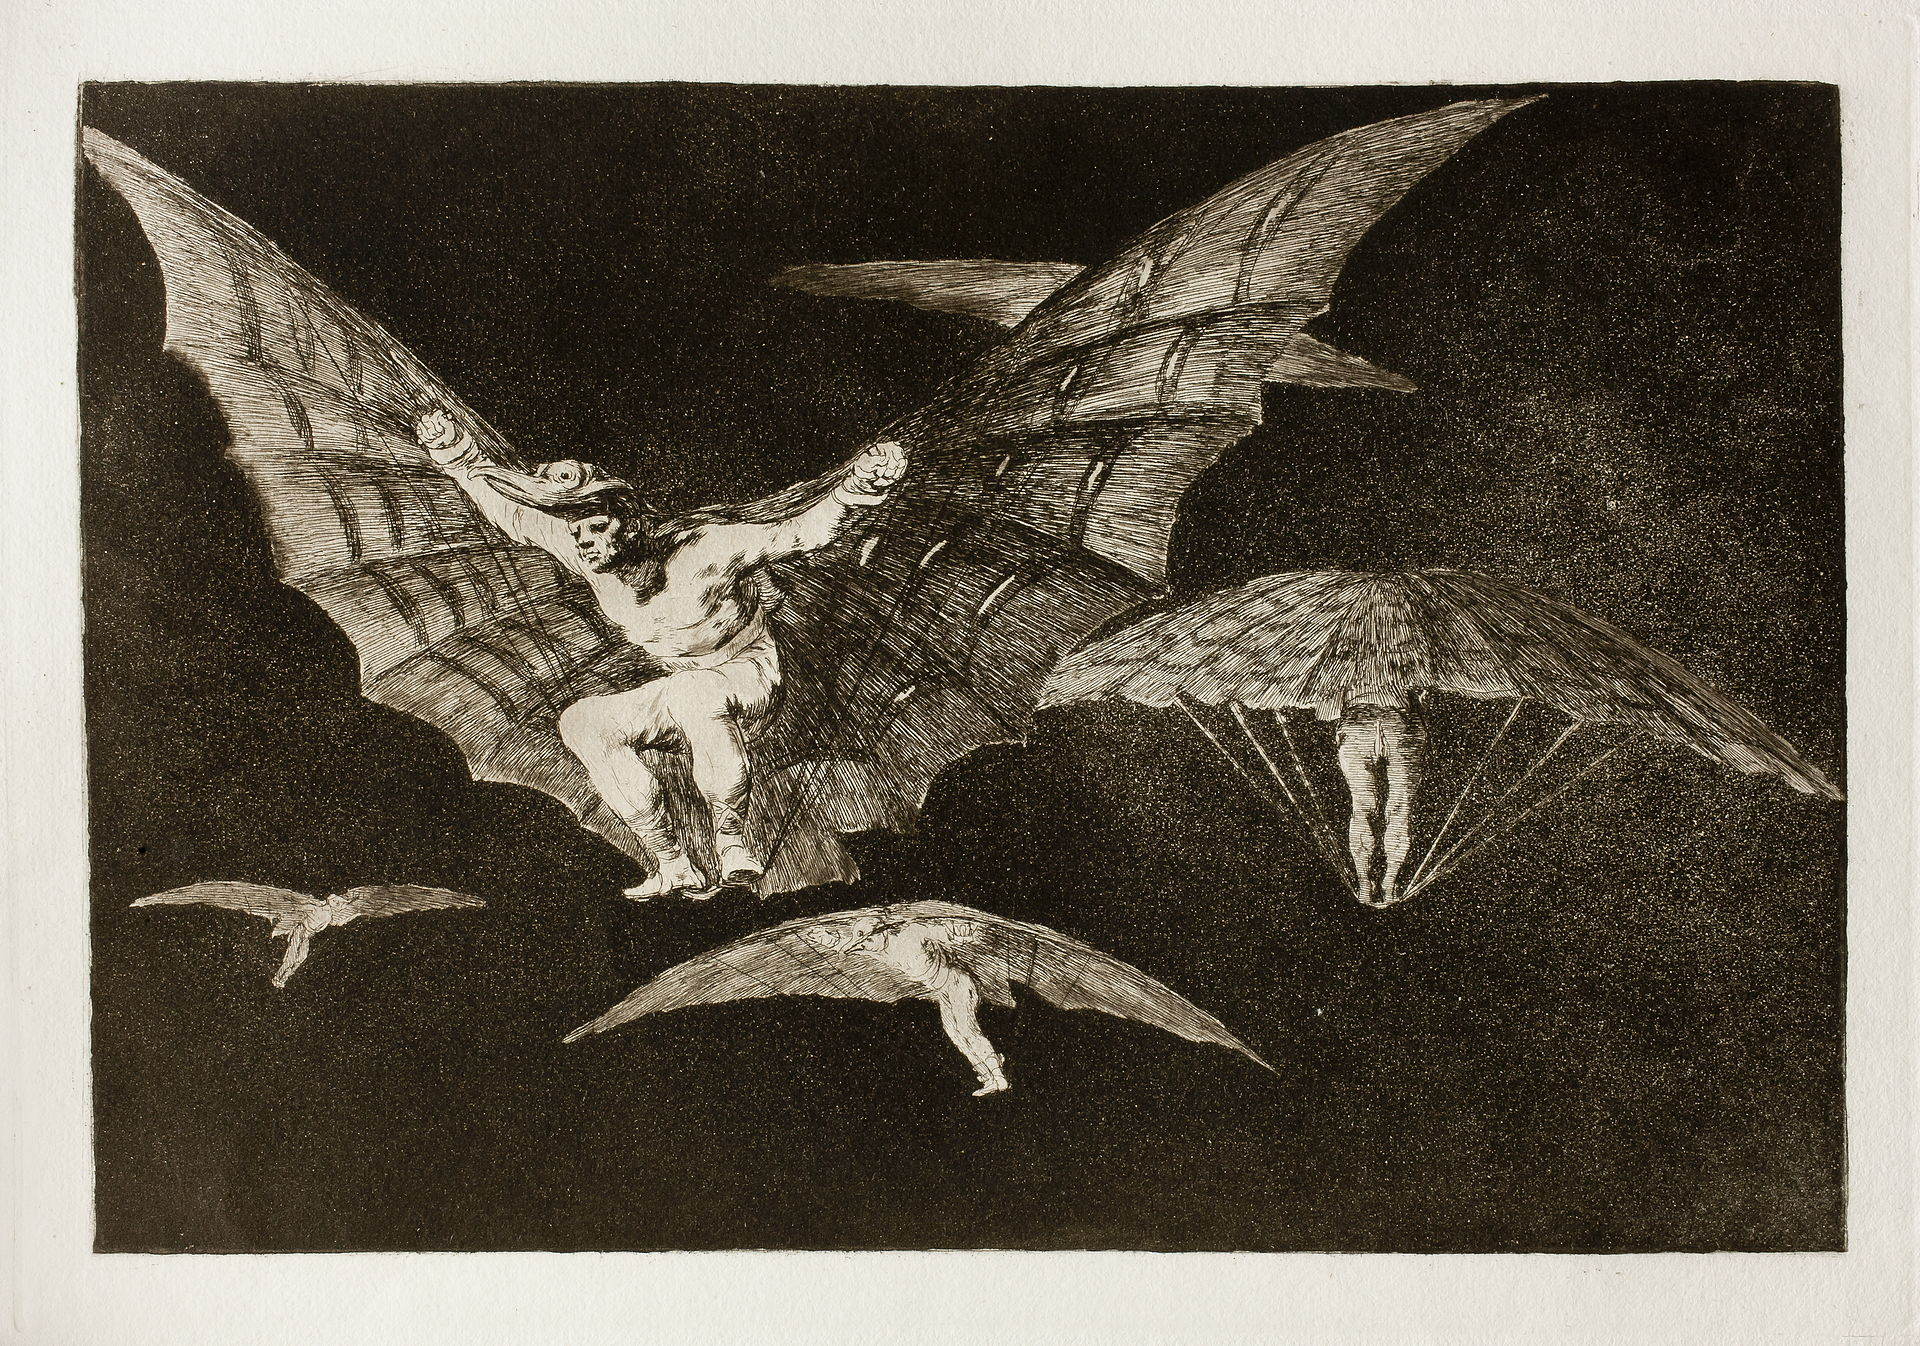
\includegraphics[width=1
		\textwidth]{goya-Modo_de_volar}
	\caption{``A way of flying'', Francisco Goya, 1815--1820, Amsterdam, Rijksmuseum.}\label{fig:goya} \end{figure}

They did not die in vain\footnote{Those ``researchers'' deserved a Darwin Award of science. The Darwin Award is satirical honours that recognise individuals who have unwillingly contributed to human evolution by selecting themselves out of the gene pool.}; Science advances when scientists are wrong. Theories must be falsifiable, and scientists cheer for their failure. When it fails, there is room for new approaches. Only when we understood the observations in animal flight from the perspective of aerodynamics, we learned to fly better than any other animal before. Science works by a ``natural selection'' of ideas, where only the fittest ones survive until a better one is born. Chaitin also points out that an idea has ``fertility'' to the extent to which it ``illuminate us, and inspires us with other ideas and suggests unsuspected connections and new viewpoints''~\cite[p. 9]{chaitin:2006}.\footnote{Moacir: and pass their gene on to children (possibly new better ones)?}\footnote{Moacir: did not get the analogy which is in the side note. }

Being a Babylonian enterprise, science has no clear path. One of the exciting facts one can learn by studying the history of science is that the most robust discoveries have arisen through the study of phenomena in human-made devices~\cite{pierce:1980}. For instance, Carnot's first and only scientific work\cite{klein:1974} gave birth to thermodynamics, which is the science that explains how steam engines work. However, steam engines came before Carnot's work and were studied by him\footnote{Moacir: please mention what was the nature and importance of his work in order for the reader to link heat engines with them.}~\cite{pierce:1980}. Thus, such human-made devices may present a simplified, small instance of more complex natural phenomena.

Another example is Information Theory. Several insights of Shannon's theory of communication were generalisations of ideas that were already present in Telegraphy. New theories in artificial intelligence can, therefore,  be developed from insights in the study of deep learning phenomena\footnote{Understanding human intelligence using artificial intelligence is a field of study called Computational Neuroscience.}.


\subsection{Bringing science to Computer Science} Despite the name, Computer Science has been more mathematics than science. We, computer scientists, are very comfortable with theorems and proofs, not much with theories.

Nevertheless, Artificial Intelligence (AI) has essentially become a Babylonian enterprise, a scientific endeavour. Thus, there is no surprise when some computer scientists still see AI with some distrust and even disdain:
\begin{itemize}
	\item Even among AI researchers, there is a trend of ``mathiness'' and speculation disguised as explanations in conference papers~\cite{lipton:2018}.
	\item There is no place for papers that unpretentiously describe surprising phenomena without trying to come up with an explanation. As if the mere inconsistency of the current theoretical framework was unworthy of publication.
\end{itemize}

While physicists rejoice in finding phenomena that contradict current theories, computer scientists get baffled. In Natural Sciences, unexplained phenomena lead to theoretical development. In AI, they bring ``winters'', periods of progress stagnation and lack of funding.\footnote{Moacir: not sure if I get this. Did you mean when some line of research is frozen until some new evidence flourishes?}.\index{ai winter}


\section{Problem}

\subsection{Has machine learning become alchemy?} Artificial Intelligence has been through several of the aforementioned ``winters''.  In 1957, Herbert Simon\footnote{Herbert Simon (1916--2001) received the Turing Award in 1975, and the Nobel Prize in Economics in 1978} famously predicted that within ten years, a computer would be a chess champion~\cite[section 1.3]{russell:2010}. It took around 40 years, in any case. Computer scientists lacked understanding of the exponential nature of the problems they were trying to solve: Computational Complexity Theory had yet to be invented.

Machine Learning Theory (computational and statistical) tries to avoid a similar trap by analysing and classifying learning problems according to the number of samples required to learn them (and the number of steps also). An honest assessment concludes it is now failing its mission. If by one hand, it leads to the development of practical machine learning algorithms like \acfp{SVM}\footnote{Moacir: define.}, by the other, it has also predicted that generalisation requires simpler models in terms of parameters, possibly delaying the development of Deep Learning for years\footnote{Moacir: other people would argue the development of DL was delayed by - lack of massive annotated data, lack of computational power, memory to handle such data}. In total disregard to the theory, deep learning models have shown spectacular generalisation power\footnote{Moacir: yes, for some domains/tasks, but even more spectacular capability of overfitting - even random labels} with hundreds of millions of parameters.

% \begin{quote}
% 	\small \textit{\flushright The curse of dimensionality is quite meaningless in practice[\ldots]\cite{howard:2018ml1}.\flushright --- Jeremy Howard, \spacedlowsmallcaps{fast.ai} creator\\
% 		\vspace{1cm} }
% \end{quote}

In the last decade, we have witnessed a myriad of astonishing successes in Deep Learning. Despite those many successes in research and industry applications, we may again be climbing a peak of inflated expectations. If, in the past, the false solution was to throw computation power on problems, today we try throwing data\footnote{Moacir: maybe both. Many SOA models are currently using ensembles of deep networks... but I get your point! in addition to the computational power, data is used in the same sense to draw conclusions that may not be reliable.}. Such behaviour has triggered a winner-takes-all competition among a handful of large corporations for who owns more data (our data), raising ethical concerns about privacy and concentration of power\cite{oneil:2016}\footnote{Moacir: maybe citing O'neil, weapons of Math Destruction or other work-related.}.

Nevertheless, we know that learning from way fewer samples is possible: humans show a much better generalisation ability than our current state of the art artificial intelligence. To achieve such needed generalisation power, we may need to understand better how learning happens in deep learning. Rethinking generalisation~\cite{zhang:2016} might reshape the foundations of machine learning theory.

\subsection{Problem statement} The practice of modern machine learning has outpaced its theoretical development. In particular, deep learning models present generalisation capabilities unpredicted by the current machine learning theory. There is yet no established new general theory of learning which handles this problem.

In 2015, Naftali Tishby and Noga Zaslavsky published a theory of learning based on the information-theoretical concept of the bottleneck principle~\cite{tishby:2015dlib}.

% This theory is general and can explain several deep learning phenomena inconsistent with the current Machine Learning Theory. The reason it is still not yet \textit{hors concours} is three-fold:
% \begin{enumerate}
% 	\item There has been some valid criticism to the experimental setting of the article mentioned above, which independent developments from~\citeauthor{achille:2017emergence}~\citeauthoritle{achille:2017emergence} address\footnote{Moacir: address?}.
% 	\item The understanding of this new theory demands prior knowledge in Information Theory to which deep learning practitioners of today are not used.
% 	\item Efforts on this new theory are scattered, and knowledge still needs to be consolidated.
% \end{enumerate}


\section{Objective}

This document aims to investigate the scattered efforts of using the information bottleneck principle to explain the generalisation capabilities of deep neural networks and consolidate them into a comprehensive digest of this new general deep learning theory.

Investigar até que ponto  IBT pode ajudar a melhor entender o Deep Learning e seus fenômenos; apresentando pontos fortes, fracos e oportunidades de pesquisa.

Perguntas de Pesquisa:
- Quais são os fundamentos da IBT? Como se diferem dos da MLT?
- É possível criar uma ponte entre MLT e IT através de IBT? Como IBT é diferente de abordagens anteriores nesse sentido como MDL?
- IBT invalida algum resultado de MLT?
- Pode IBT explicar fênomenos ainda pouco compreendidos?

Perguntas:
Quais são os fundamentos da IBT? Como se diferem dos da MLT?
É possível criar uma ponte entre MLT e IT através de IBT? Como IBT é diferente de abordagens anteriores nesse sentido como MDL?
Metodologia:
Derivar a partir de uma definição de inteligência tanto MLT, quanto IBT e identificar diferenças de  suposições.
Resultados Esperados:
Uma “árvore genealógica” das duas teorias e quadro comparativo.
Demonstração do conceito “fator de Occam” da perspectiva Bayesiana como sendo uma medida de informação.
Comparação IBT vs. MDL

Perguntas:
IBT invalida algum resultado de MLT?
Pode IBT explicar fênomenos ainda pouco compreendidos?
Metodologia:
A partir de uma lista de fenômenos compreendidos e não compreendidos, apontar diferenças entre a perspectiva atual e a da IBT.
Resultados Esperados:
As explicações correntes de MLT continuam válidas em IBT;
IBT pode explicar alguns aspectos de fenômenos ainda mal compreendidos.



\section{Outline}

The dissertation is organised in two parts:\\
PART I - Background:
\begin{itemize}
	\item Chapter 2--Artificial Intelligence: The chapter defines what artificial intelligence is, presents the epistemological differences of intelligent agents in history, and discusses their consequences to machine learning theory.
	\item Chapter 3 --- Probability Theory: The chapter derives propositional calculus and probability theory from a list of desired characteristics for sceptical agents.
	\item Chapter 4 --- Information Theory: The chapter derives Shannon Information from Probability Theory, explicates some implicit assumptions, and explains basic Information Theory concepts.
	\item Chapter 5 --- Machine Learning Theory: The chapter presents the theoretical framework of Machine Learning, the PAC model, theoretical guarantees for generalisation, and expose criticism due to its lack of explanation on Deep Learning phenomena.
	\item Chapter 6 --- Proposal: The chapter presents the plan for finishing the dissertation.
\end{itemize}

PART II --- An Information Theory of Deep Learning
\begin{itemize}
	\item Chapter 5 - The plan: In wich we present a plan to the dissertation.
 \end{itemize}
